\section{Performances}

\subsection{Environnement de test}

\subsubsection{Spécifications matérielles}

Les mesures ont été effectuées sur la machine suivante :

\begin{itemize}
    \item \textbf{Processeur} : AMD Ryzen 7 5700U (8 cœurs physiques, 16 threads logiques, jusqu'à 4,37 GHz)
    \item \textbf{Caches} : L1d/L1i 256 Kio $\times$ 8, L2 4 Mio $\times$ 8, L3 8 Mio
    \item \textbf{Mémoire RAM} : 16 Go
    \item \textbf{Système} : Linux x86\_64
\end{itemize}

\subsubsection{Conditions d'exécution}

Afin d'obtenir des mesures reproductibles et comparables :

\begin{itemize}
    \item Chaque binaire est épinglé sur un \textbf{seul cœur} (cœur 0) via \texttt{taskset -c 0},
          éliminant les migrations de tâches et les effets de cache inter-cœurs.
    \item Chaque configuration est exécutée \textbf{10 fois} (\texttt{RUNS = 10}) ;
          on rapporte la \textbf{moyenne} et l'\textbf{écart-type} sous forme de barres d'erreur.
    \item Les temps sont mesurés à l'intérieur du binaire et émis sur la sortie standard
          sous la forme \texttt{GRAPH;<temps en µs>}, puis convertis en millisecondes.
\end{itemize}

Deux tests ont été retenus pour l'évaluation :
\begin{itemize}
    \item \texttt{21-create-many} : crée et détruit $n$ threads séquentiellement,
          ce qui sollicite intensivement l'allocation et la libération mémoire.
    \item \texttt{31-switch-many} : crée $n$ threads effectuant chacun 50 \texttt{thread\_yield},
          ce qui génère un grand nombre de changements de contexte.
\end{itemize}
Ces deux tests couvrent les deux axes de performance les plus significatifs
d'une bibliothèque de threads.

Les graphes sont générés automatiquement par \texttt{scripts/plot.py} via \texttt{make graphs}.

\subsection{Vue d'ensemble : pthreads vs bibliothèque utilisateur}

Le premier graphe compare toutes les variantes de notre bibliothèque avec les \textbf{pthreads POSIX}.

\begin{figure}[H]
    \centering
    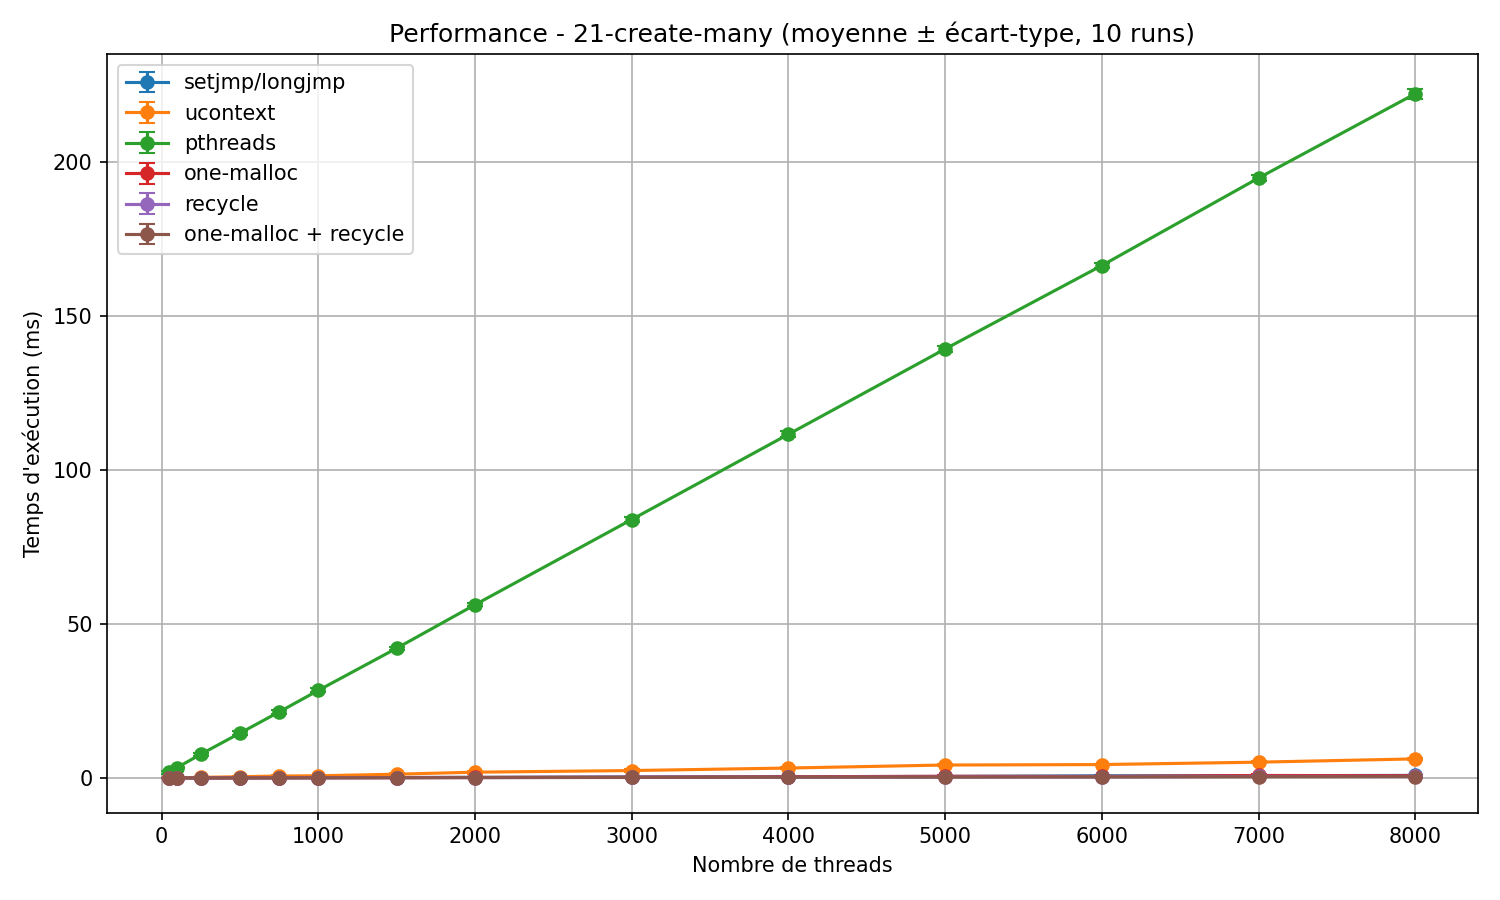
\includegraphics[width=0.7\textwidth]{rapport-final/images/21-create-many-pthread.png}
    \caption{Création/destruction de $n$ threads : toutes variantes + pthreads.}
\end{figure}

\begin{figure}[H]
    \centering
    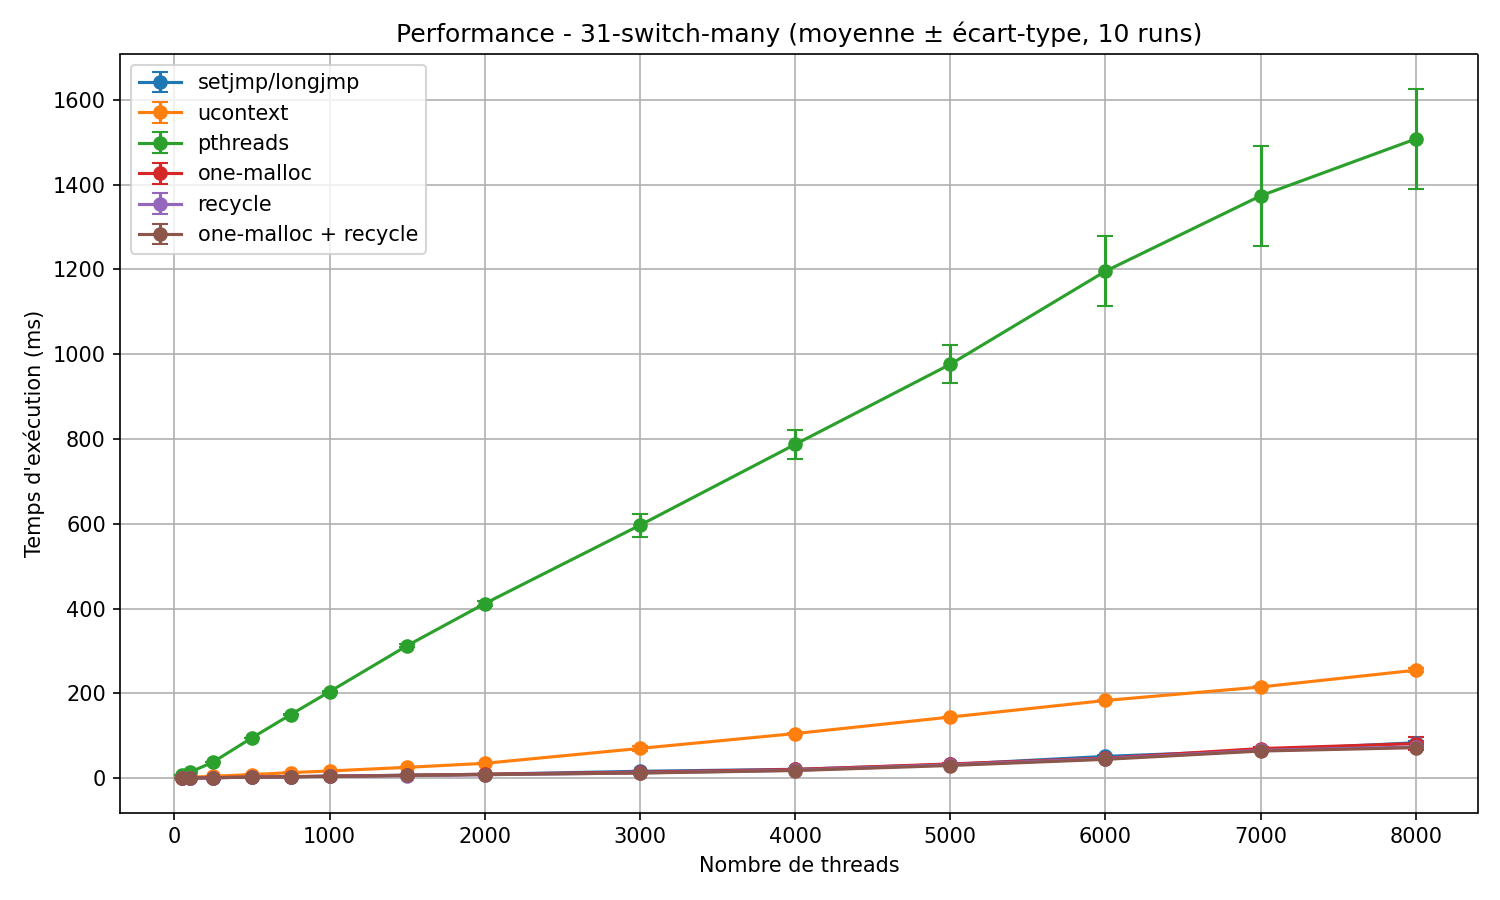
\includegraphics[width=0.7\textwidth]{rapport-final/images/31-switch-many-pthread.png}
    \caption{Changements de contexte ($n$ threads $\times$ 50 yields) : toutes variantes + pthreads.}
\end{figure}

Les pthreads se révèlent nettement plus lents que toutes nos variantes.
Cela s'explique par leur nature de \textbf{threads noyau} : chaque création passe
par l'appel système \texttt{clone}, et chaque changement de contexte implique une
transition espace utilisateur/noyau via l'ordonnanceur du système.
Notre bibliothèque opère entièrement en espace utilisateur, supprimant ces
transitions coûteuses au prix d'un ordonnancement coopératif.

Ces benchmarks sont toutefois réalisés sur un \textbf{seul cœur}, ce qui défavorise
structurellement les pthreads. Pour le confirmer, les graphes suivants répètent les mêmes mesures \textbf{sans épingler
le processus sur un seul cœur} (sans \texttt{taskset}). Les pthreads voient leurs
performances nettement améliorées et se rapprochent significativement de notre
variante \texttt{ucontext}, illustrant l'impact du parallélisme noyau dès que
le système d'exploitation peut librement distribuer les threads sur plusieurs cœurs.

\begin{figure}[H]
    \centering
    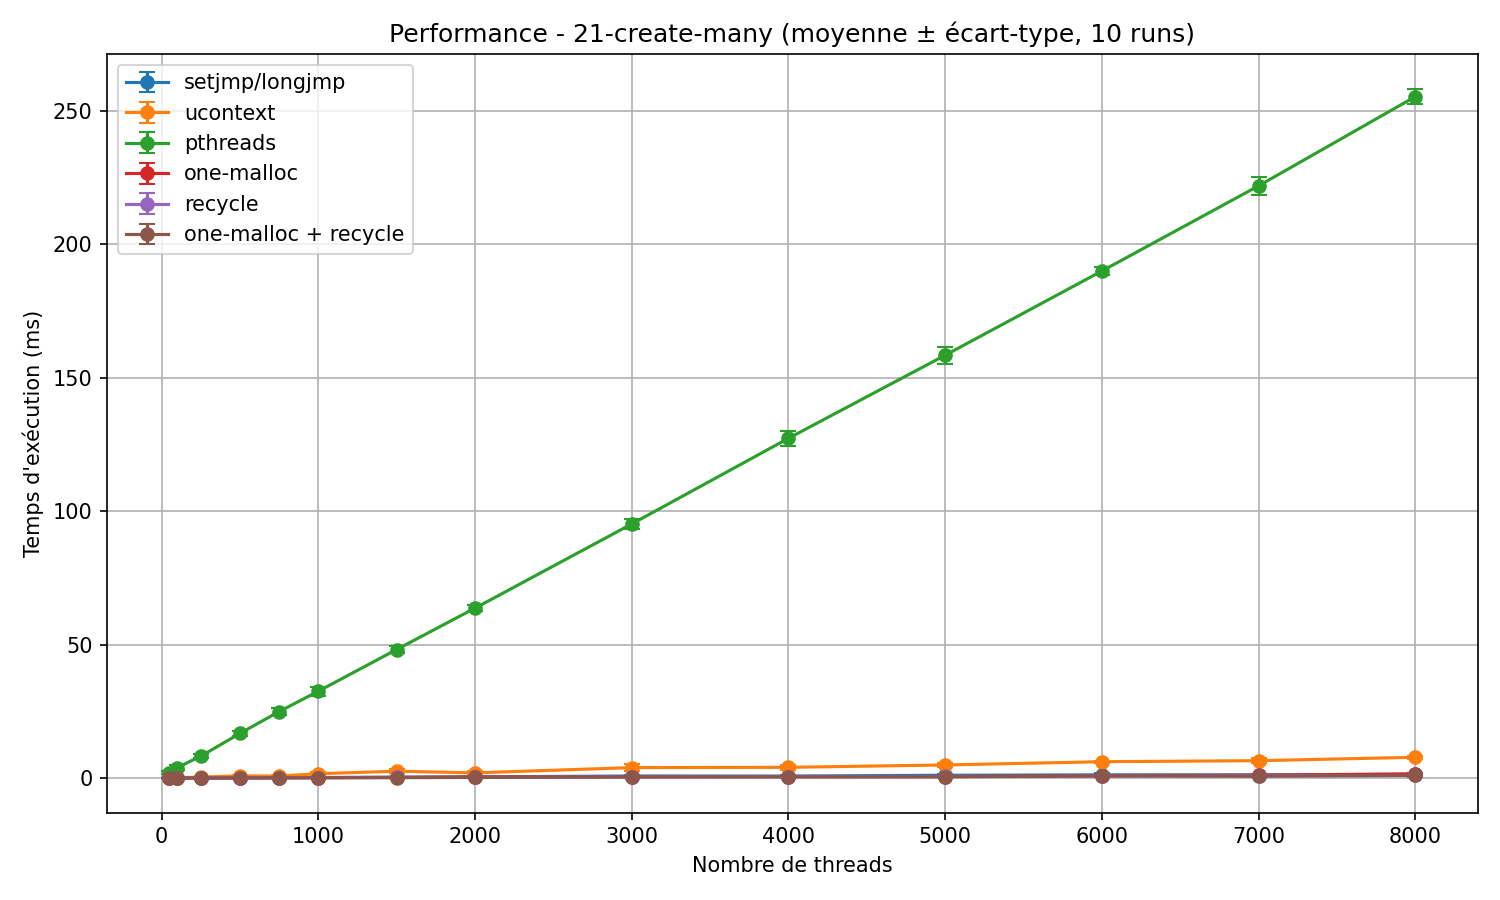
\includegraphics[width=0.7\textwidth]{rapport-final/images/21-create-many-no-taskset.png}
    \caption{Création/destruction de $n$ threads sans \texttt{taskset} : pthreads vs bibliothèque utilisateur.}
\end{figure}

\begin{figure}[H]
    \centering
    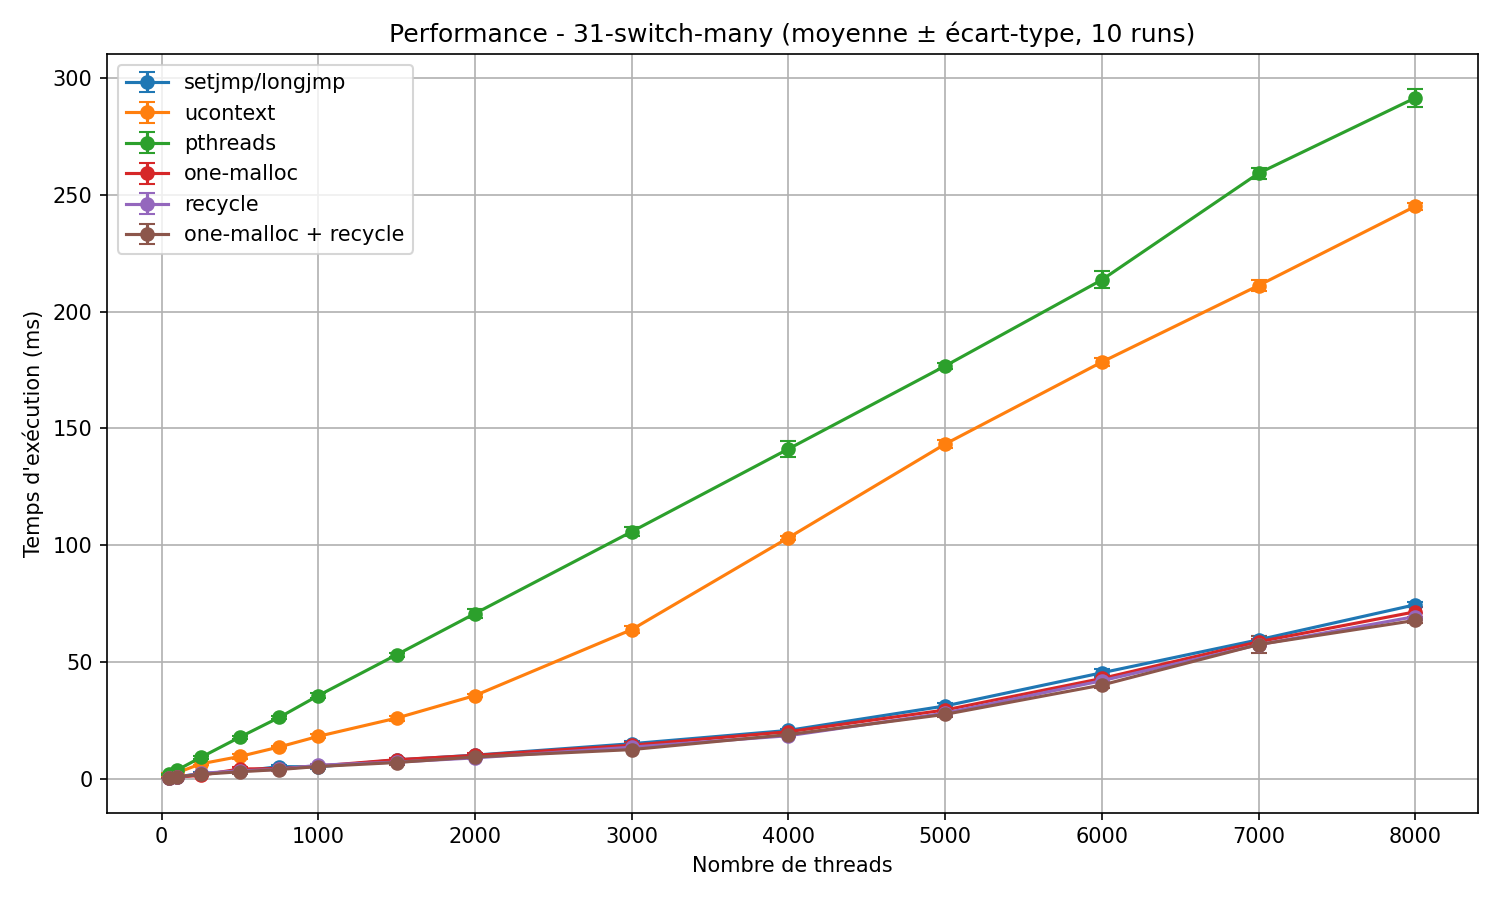
\includegraphics[width=0.7\textwidth]{rapport-final/images/31-switch-many-no-taskset.png}
    \caption{Changements de contexte sans \texttt{taskset} : pthreads vs bibliothèque utilisateur.}
\end{figure}

\subsection{Comparaison \texttt{ucontext} vs \texttt{setjmp/longjmp}}

En retirant les pthreads du graphe, les différences entre nos variantes deviennent visibles.

\begin{figure}[H]
    \centering
    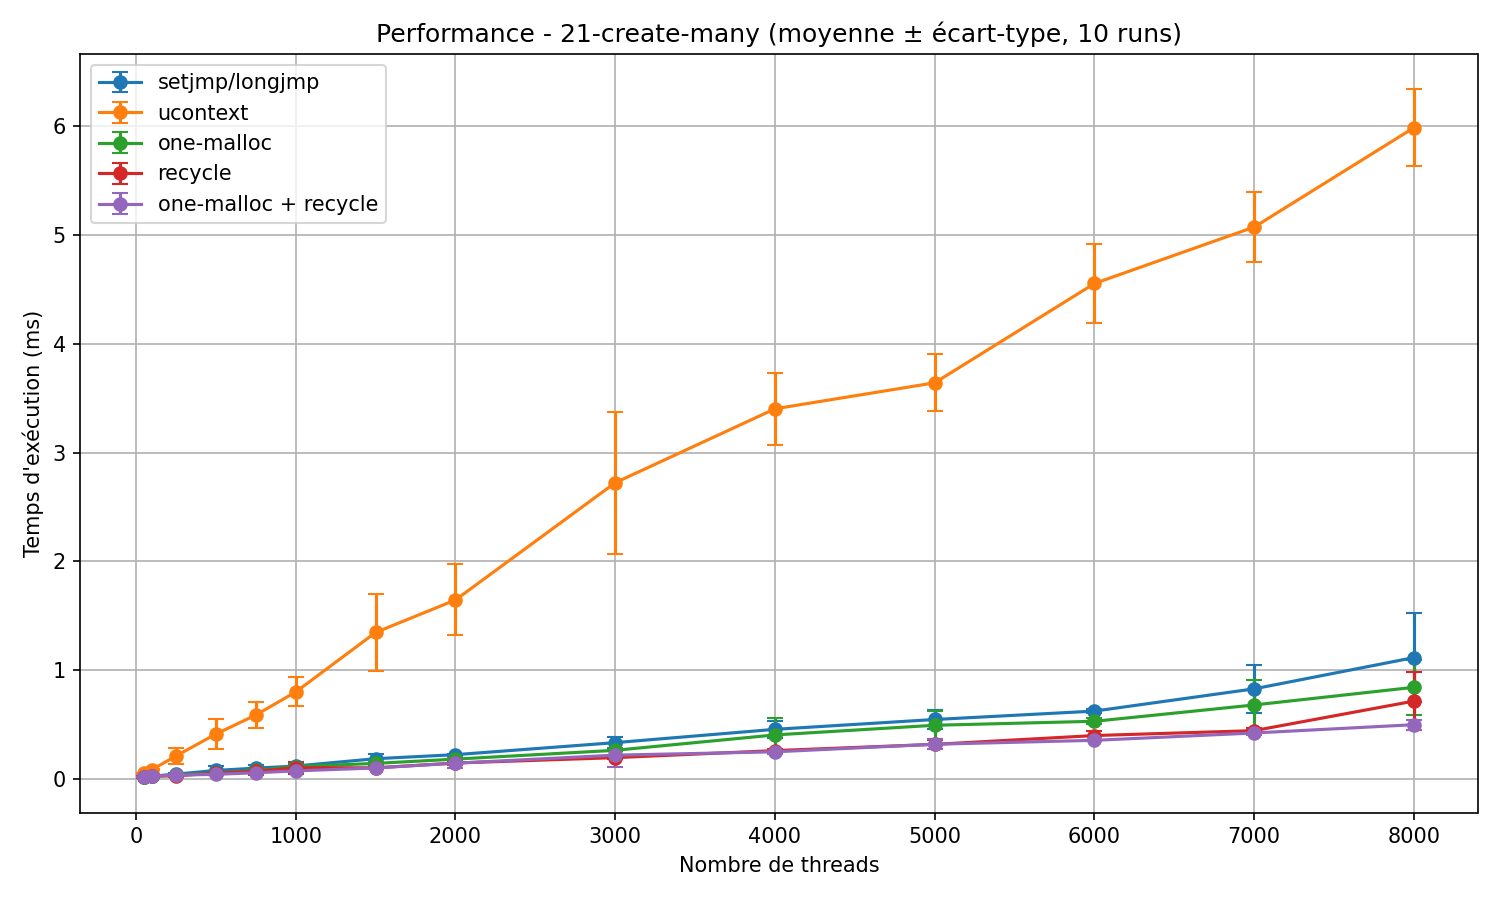
\includegraphics[width=0.7\textwidth]{rapport-final/images/21-create-many-context.png}
    \caption{Création/destruction : ucontext vs variantes setjmp/longjmp.}
\end{figure}

\begin{figure}[H]
    \centering
    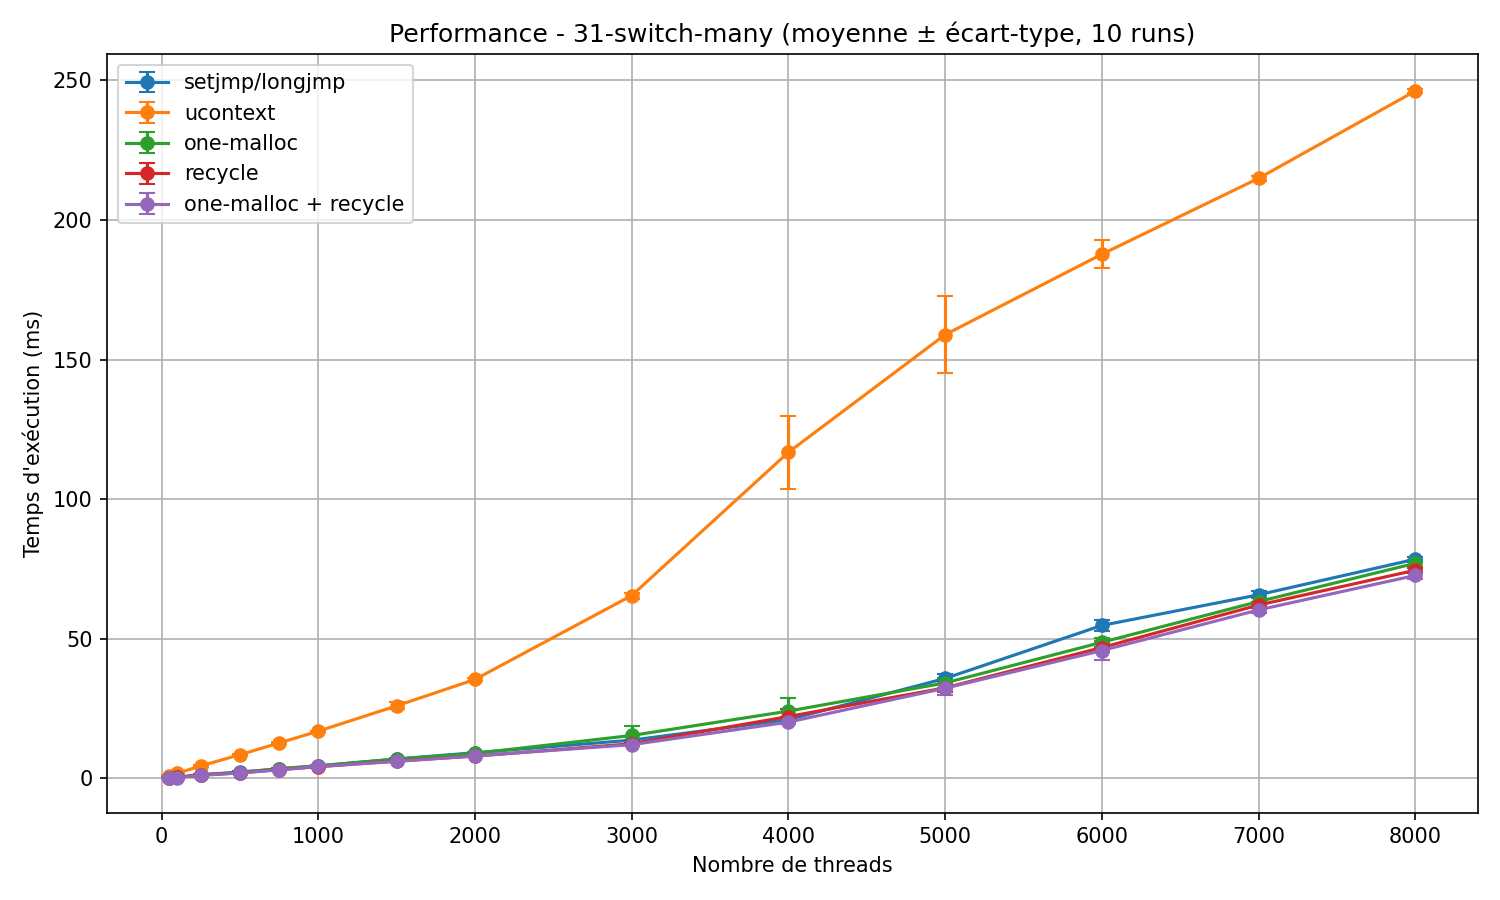
\includegraphics[width=0.7\textwidth]{rapport-final/images/31-switch-many-context.png}
    \caption{Changements de contexte : ucontext vs variantes setjmp/longjmp.}
\end{figure}

La variante \texttt{ucontext} (\texttt{makecontext}/\texttt{swapcontext}) est plus lente
que les variantes \texttt{setjmp/longjmp}. En effet, \texttt{swapcontext} sauvegarde
l'intégralité du contexte d'exécution, y compris le \textbf{masque de signaux POSIX},
ce qui implique un appel système supplémentaire à chaque changement de contexte.
\texttt{setjmp/longjmp} se contente de sauvegarder le compteur de programme,
le pointeur de pile et quelques registres essentiels, évitant cet appel système.

\subsection{Impact des optimisations mémoire}

En retirant également \texttt{ucontext}, on peut comparer finement les quatre
variantes \texttt{setjmp/longjmp} entre elles.

\begin{figure}[H]
    \centering
    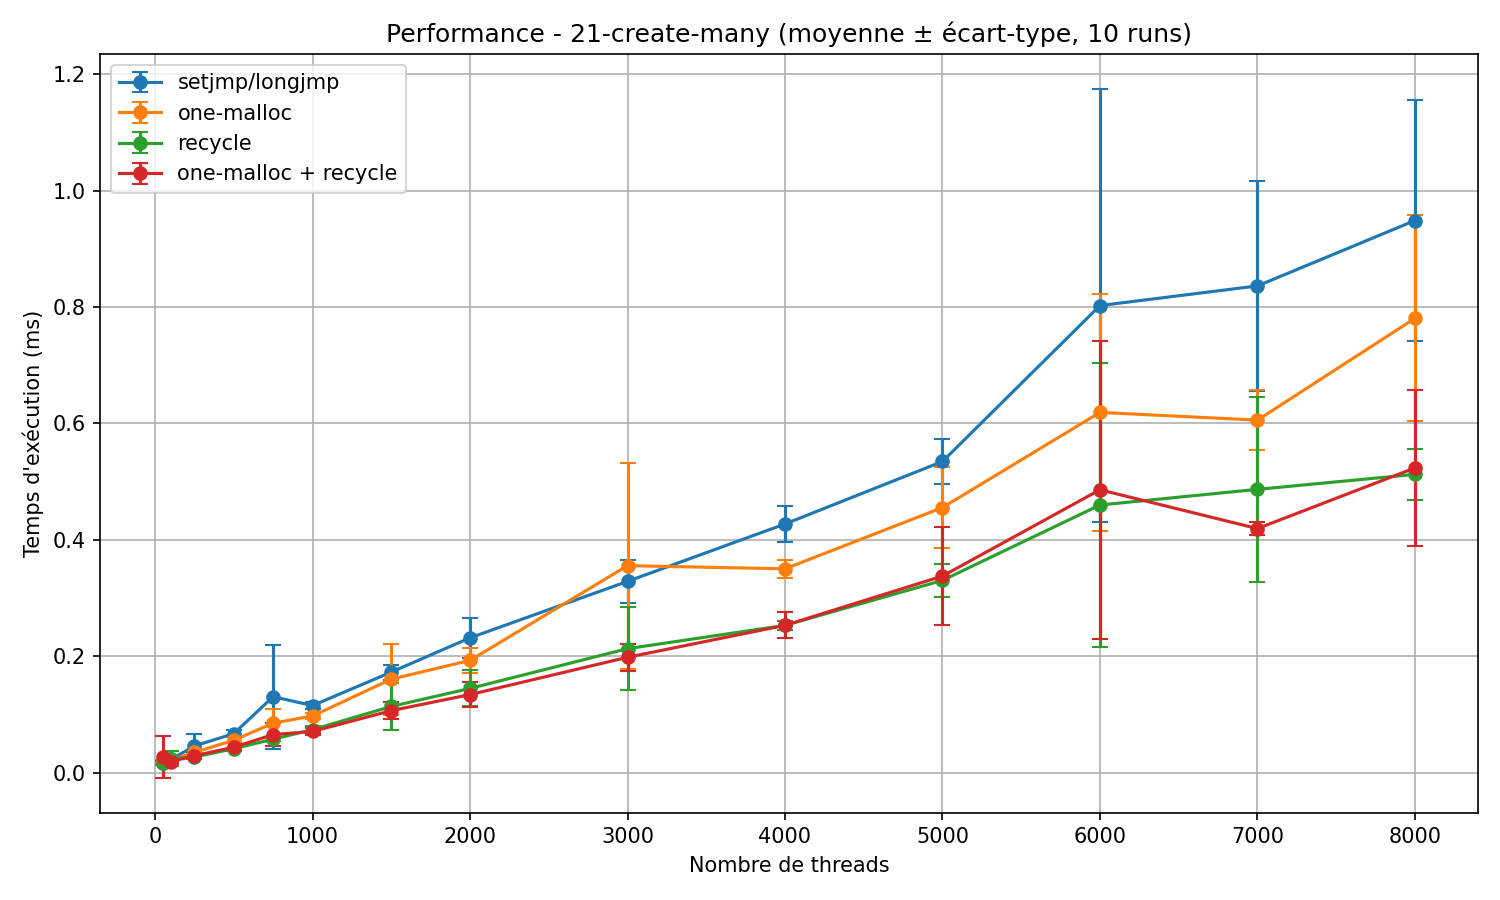
\includegraphics[width=0.7\textwidth]{rapport-final/images/21-create-many-optim.png}
    \caption{Optimisations mémoire : création/destruction de threads.}
\end{figure}

\begin{figure}[H]
    \centering
    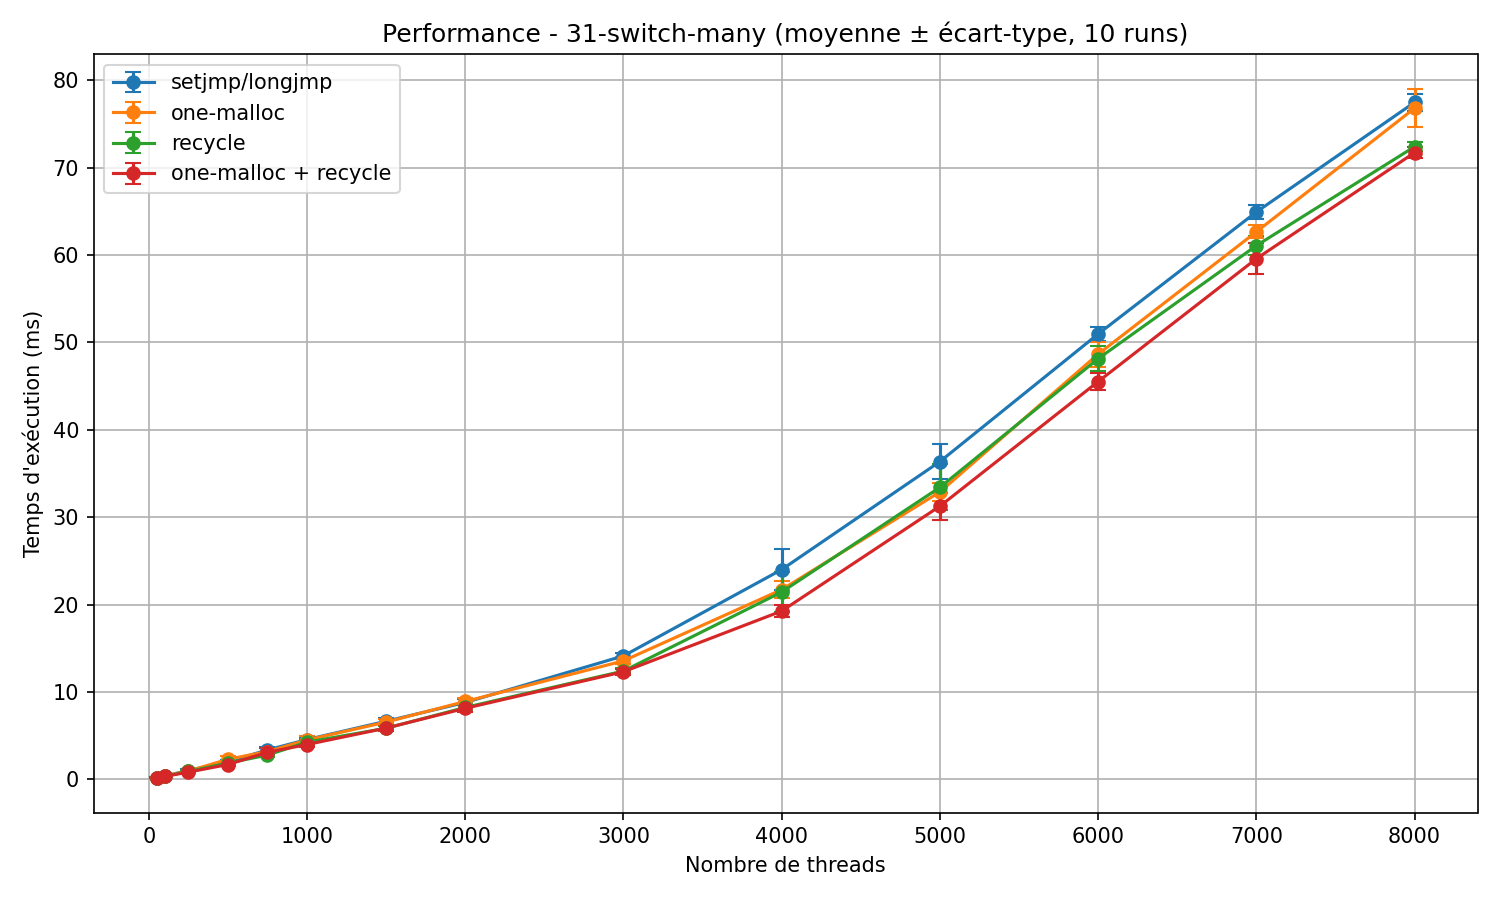
\includegraphics[width=0.7\textwidth]{rapport-final/images/31-switch-many-optim.png}
    \caption{Optimisations mémoire : changements de contexte.}
\end{figure}

\begin{itemize}
    \item \textbf{setjmp/longjmp} : deux \texttt{malloc} séparés (structure + pile), version de référence.
    \item \textbf{one-malloc} : structure et pile allouées en un seul bloc contigu (\texttt{-DUSE\_ONE\_MALLOC}),
          réduisant la fragmentation et améliorant la localité de cache.
    \item \textbf{recycle} : file de réutilisation des blocs libérés (\texttt{-DUSE\_RECYCLE}),
          évitant les appels répétés à \texttt{malloc}/\texttt{free}.
    \item \textbf{one-malloc + recycle} : combinaison des deux optimisations, version la plus performante.
\end{itemize}

Ces optimisations portent exclusivement sur l'allocation et la libération mémoire des threads.
Elles n'ont donc d'impact que lors de la \textbf{création et destruction} de threads :
sur le test \texttt{31-switch-many}, les quatre courbes se superposent quasiment,
car tous les changements de contexte utilisent les mêmes mécanismes indépendamment
de la stratégie d'allocation.

En revanche, sur le test \texttt{21-create-many}, les différences sont nettes.
La variante \textbf{one-malloc} réduit de moitié le nombre d'appels à
\texttt{malloc}/\texttt{free} en regroupant structure et pile dans un seul bloc,
ce qui se traduit par un gain visible mais modéré.
La variante \textbf{recycle} va plus loin : en réutilisant les blocs déjà alloués,
elle supprime presque entièrement les appels système liés à l'allocation dès que
les threads sont créés et détruits en boucle, ce qui en fait l'optimisation
la plus impactante.
La version \textbf{one-malloc + recycle} combine les deux et reste très proche
de la version recycle seule, ce qui confirme que le recyclage est l'optimisation
dominante et la plus puissante.
